\chapter{Вступ}
\section{Теоретичні відомості до першого завдання}
\subsection{Алгебра логіки}
\textbf{Алгебра логіки} \emph{(Булева логіка, двійкова логіка, двійкова алгебра)} — розділ математичної логіки, що вивчає систему логічних операцій над висловлюваннями. Вважається, що висловлювання можуть бути тільки істинними або помилковими, тобто використовується так звана \emph{бінарна або двійкова логіка}.

Булева функція задається у вигляді таблиці, або графіка зі стандартним (лексикографічним) розташуванням наборів аргументів,виконана кодом Грея.

\textbf{Код Грея} — одна із систем кодування інформації, в якій два послідовні коди відрізняються значенням лише одного біта.

\textbf{Таблиця істинності} — математична таблиця, що широко використовується у математичній логіці зокрема в алгебрі логіки, численні висловлень для обчислення значень булевих функцій.

Приклад таблиці істинності:
\begin{center}
\begin{table}[h!]
\begin{tabu}{ | X[-3,l] | X[-3,l] | X[-3,l] | X[-3,l] |}
\hline
N &$X_{1}$ & $X_{2}$ & $F_{1}$ \\
 \hline
0 & 0 & 0 & 0  \\
\hline
1 &  0 & 1  &  0  \\
\hline
2 & 1 & 0 & 0   \\
\hline
3 & 1 & 1 & 1  \\
\hline
\end{tabu}
\vspace{6mm}\\
\caption{Приклад таблиці істинності}\label{tab:logic_truth_table_ex}
\end{table}
\end{center}
\newpage
\subsection{Базові логічні функції}
Відомі такі основні логічні функції, як:
\begin{itemize}
	\item Інверсія (логічне  'НЕ', NOT,$\lnot$)
	\begin{figure}[h!]
 	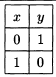
\includegraphics[scale=1]{inverter_tt.png}
 	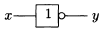
\includegraphics[scale=1]{inverter_sign.png}
 	\centering
	\caption{Інверсія}\label{fig:inverter}
	\end{figure}
	\item Кон'юнкція (логічне множення, логічне  І, AND,$\wedge$)
	\begin{figure}[h!]
 	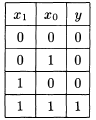
\includegraphics[scale=1]{and_tt.png}
 	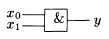
\includegraphics[scale=1]{and_sign.png}
 	\centering
	\caption{Кон'юнкція}\label{fig:and}
	\end{figure}
	\item Диз'юнкція (логічне додавання, логічне  АБО, OR,$\lor$)
	\begin{figure}[h!]
 	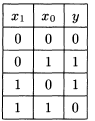
\includegraphics[scale=1]{or_tt.png}
 	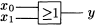
\includegraphics[scale=1]{or_sign.png}
 	\centering
	\caption{Диз'юнкція}\label{fig:or}
	\end{figure}
	\item Виключне 'АБО'(Сума по модулю 2,mod2,XOR,$\oplus$)
	\begin{figure}[h!]
 	\includegraphics[scale=1]{xor_tt.png}
 	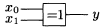
\includegraphics[scale=1]{xor_sign.png}
 	\centering
	\caption{Виключне 'АБО'}\label{fig:xor}
	\end{figure}
\end{itemize}
Також існують логічні функції для базисів(детально розглядаються на сторінці  \pageref{subsect:logic_basis}).
\newpage
\subsection{Форма подання логічних виразів}
Логічний вираз можна подати у трьох формах:
\begin{itemize}
	\item Диз'юнктивна нормальна форма (ДНФ);
	\item Кон'юнктивна нормальна форма (КНФ);
	\item Алгебраїчна нормальна форма (АНФ або поліном Жегалкіна)(не розглядається в даній роботі).
\end{itemize}

\textbf{Диз'юнктивна нормальна форма (ДНФ)}в булевій логіці — нормальна форма 	в якій булева формула має вид диз'юнкції декількох кон'юнктів (де кон'юнктами 			називаються кон'юнкції декількох пропозиційних символів або їх заперечень).
	
\textbf{Доскона́лою диз'юнкти́вною норма́льною фо́рмою (ДДНФ)} булевої функції 				називається диз'юнкція тих конституент одиниці, які перетворюються в одиницю на тих 	самих наборах змінних, що й задана функція. ДДНФ повинна задовольняти наступним 		умовам:
\begin{itemize}
\item в ній немає однакових доданків;
\item жоден із доданків не містить двох однакових співмножників;
\item жоден із доданків не містить змінну разом із її запереченням;
\item в кожному окремому доданку є як співмножник або змінна $x_{i}$, або її заперечення для будь-якого $i = 1, 2, …, n$.
\end{itemize}

\textbf{Кон'юнкти́вна норма́льна фо́рма (КНФ)} в булевій логіці - нормальна форма в якій булева формула має вид кон'юнкції декількох диз'юнктів (де диз'юнктами називаються диз'юнкції декількох пропозиційних символів або їх заперечень). Кон'юнктивна нормальна форма широко використовується в автоматичному доведенні теорем, зокрема вона є основою для використання правила резолюції.

\textbf{Досконалою кон’юнктивною нормальною формою (ДКНФ)} булевої функції називається кон’юнкція тих конституент нуля, які перетворюються в нуль на тих самих наборах змінних, що й задана функція. Також по аналогії з ДДНФ, будь-яка булева функція має одну ДКНФ (кількість її членів дорівнює кількості нульових значень функції) і декілька КНФ. Можна навести такі властивості ДКНФ, що виділяють її з усіх КНФ:
\begin{itemize}
\item в ній немає однакових співмножників;
\item жоден із співмножників не містить двох однакових доданків;
\item жоден із співмножників не містить якої-небудь змінної разом з її запереченням;
\item в кожному окремому співмножнику є як складова або змінна $x_{i}$, або її заперечення для будь-якого $i=1,2,…,n$.
\end{itemize}
\subsection{Дії над логічними виразами}
Для логічних виразів існують такі закони алгебри:
\begin{center}
\begin{table}[h!]
\begin{tabu} { | X[3,с] | X[3,c] | X[3,c] | }
 \hline
Назва закону& АБО & І \\
 \hline
 Переміщення &$A \lor B = B \lor A$  &$A \wedge B = B \wedge A $  \\
\hline
 Комбінування &$A \lor (B \lor C)= (A \lor B) \lor C $  &$A \wedge (B \wedge C)= (A \wedge B) \wedge C $  \\
\hline
Розподільний &$(A \lor B) \wedge C= A \wedge C \lor B \wedge C $  \vspace{1mm}&$(A \wedge B) \lor C= A \lor C \wedge B \lor C $ \vspace{1mm}   \\
\hline
Правило де Моргана & $\neg(A \lor B) = \neg A \wedge \neg B$& $\neg(A \wedge B) = \neg A \lor \neg B$\\
\hline
Ідемпотентність & $A \lor A = A$ &$A \wedge A = A $   \\
\hline
Виключення &$A \lor \neg A = 1$ & $A \wedge \neg A = 0$  \\
\hline
Операції з константами & $A \lor 1= 1$;$A \lor 0 = A$&$A \wedge 1 = A$;$A \wedge 0 = 0$  \\
\hline
Поглинання &$A \lor (A \wedge B) = A $ &$A \wedge (A \lor B) = A $   \\
\hline
Склеювання&$(A \wedge B) \lor (\neg A \wedge B)=B$&$(A \lor B) \wedge (\neg A \lor B)=B$   \\
\hline
\end{tabu}
\vspace{6mm}\\
\caption{Таблиця законів алгебри логічних виразів}\label{tab:logic_formulas}
\end{table}
\end{center}

\newpage
\subsection{Мінімізація логічних виразів}
\textbf{Мінімізація булевих функцій} — спрощення булевих виразів. Оскільки логічні функції реалізують за допомогою певного набору пристроїв, то, спрощуючи вираз, зменшуємо кількість елементів.

Існують такі методи мінімізації:
\begin{itemize}
	\item метод Блейка-Порецького;
	\item метод Нельсона;
	\item метод Дужкових форм;
	\item метод Карта Карно;
	\item метод Куайна — Мак-Класкі.
\end{itemize}

В данному проекті буде розглянутий тільки метод Блейка-Порецького та метод Нельсона.

\textbf{Метод Блейка-Порецького та Нельсона}

Алгоритм мінімізації за методами Блейка-Порецького та Нельсона полягає в:
\begin{enumerate}
\item Виконати всі можливі склеювання виразів;
\item Виконати всі можливі поглинання виразів;
\item Виконати перевірку виразу на слеювання і поглинання;
\item Повторити пунтки 1-3 до отримання мінімального варінту виразу.
\end{enumerate}

\newpage
\subsection{Логічні базиси}\label{subsect:logic_basis}
\textbf{Функціонально повним набором або логічним базисом} - називається набір логічних операцій, що дозволяє аналітично описати будь-яку логічну функцію.Такий набір складають основні логічні операції АБО, І, НЕ, тому він є одним з логічних базисів.

Логічний базис називається \textbf{мінімальним}, якщо видалення з набору хоча б однієї операції перетворює його в функціонально неповний.

 Логічний базис НЕ, АБО, І не є мінімальним, так як на підставі законів подвійності можна виключити з логічних виразів операцію АБО або І, отже, він є надлишковимбазисом. Мінімальний базис складають дві операції НЕ, АБО і НЕ, І. 
 
Практичного уваги заслуговують мінімальні базиси, що представляють собою тільки одну операцію. До них відносяться операції \emph{логічного множення з запереченням (І-НЕ, штрих Шеффера,NAND,$\uparrow$,$\bar{\wedge}$) і логічного додавання з запереченням (АБО-HE, стрілка Пірса,NOR,$\downarrow$,$\bar{\vee}$)}.

\begin{figure}[h!]
 	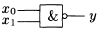
\includegraphics[scale=1]{nand_sign.png}
 	\centering
	\caption{Умовне позначення І-НЕ}\label{fig:nand}
\end{figure}
\begin{figure}[h!]
 	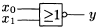
\includegraphics[scale=1]{nor_sign.png}
 	\centering
	\caption{Умовне позначення АБО-НЕ}\label{fig:nor}
\end{figure}	

\newpage
\section{Теоретичні відомості до другого завдання}
\subsection{Дешифратор}
\textbf{Дешифратор або декокдер} (англ. \emph{decoder}) — логічний пристрій, який перетворює код числа, що поступило на вхід, в сигнал на одному з його виходів.

Якщо число представлено у вигляді $n$ двійкових розрядів, то дешифратор повинен мати $2^{n}$ виходів.

Дешифратор довільної складності може бути складено з трьох базових логічних елементів: кон'юнкції, диз'юнкції та інверсії.
\begin{figure}[h!]
 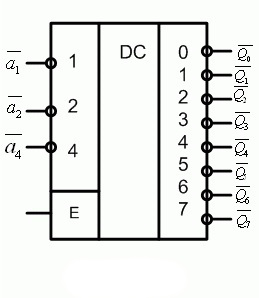
\includegraphics{decoder.jpg}
 \centering
\caption{Графічне позначення дешифратора}\label{fig:decoder}
\end{figure}
\begin{figure}[h!]
 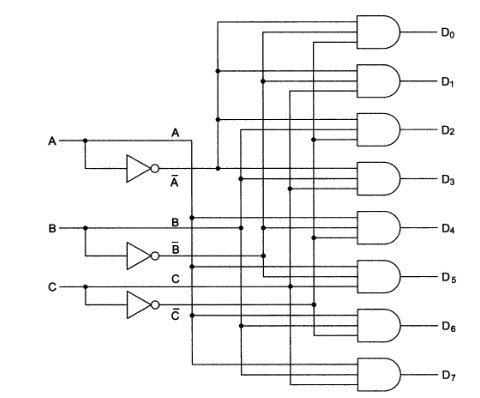
\includegraphics[scale=0.5]{decoder_scheme.png}
 \centering
\caption{Схема дешифратора з 3 входами и 8 виходами}\label{fig:decoder_scheme}
\end{figure}
\newpage
\subsection{Алгоритм побудови багатоступеневого дешифратора}
\textbf{Багатоступеневий дешифратор} — це дешифратор подуванний на основі існуючих мікросхем.Як правило не всі виходи таких дешифраторів використовуються, тобто будуються вони з обмеженою кількістю виходів.Дешифратори з обмеженою кількістю виходів, називають \textbf{неповними}.

Побудова  таких багатоступеневих дешифраторів полягає в наступному:
Нехай необхідно побудувати $N$-входовий дешифратор на основі  $K_{1}$-, $K_{2}$-, $K_{3}$- входових дешифраторів  ($N > (K_{1},K_{2},K_{3}$). 
\begin{enumerate}
\item Визначаємо кількість ступенів  $L$ виходячи з виразу (\ref{eq:decoder_N})
Числа $l_{1},l_{2},l_{3}$ визначаються підбором. 
\begin{equation}\label{eq:decoder_N}
N=l_{1}K_{1}+l_{2}K_{2}+l_{3}K_{3}
\end{equation}
Тоді загальна кількість ступенів дешифратора.
\begin{equation}\label{eq:decoder_L}
L=l_{1}+l_{2}+l_{3}
\end{equation}
Числа $l_{i}$ визначають кількість ступенів багатоступеневого дешифратора, які будуть реалізовані на основі $K_{i}$- входових дешифраторів.
\item  Визначаємо тип мікросхеми,  на основі якої будується той чи інший ступінь дешифратора. Вибір проводиться довільно враховуючи (\ref{eq:decoder_N})  і  (\ref{eq:decoder_L}).
\item Алгоритм побудови дешифратора полягає в наступному:
\begin{enumerate}
\item 1-й ступінь містить в собі 1 дешифратор(\ref{eq:decoder_n1}), тип якого визначений в кроці 2. На адресні входи цього дешифратора  подаються  старші адресні входи  дешифратора, який проектується. На $E$-вхід подається сигнал загального дозволу роботи дешифратора.
\item 2-й ступінь містить в собі  $2^{mi}$ дешифраторів по типу, визначеному в кроці 2($mi$ – кількість адресних входів попереднього ступеня, $2^{mi}$ – кількість виходів попереднього ступеня. На адресні входи всіх дешифраторів  подаються наступні після 1-го ступеню адресні входи  дешифратора, який проектується. $E$-входи дешифраторів цього ступеню підключаються до виходів попереднього ступеня.
\item Всі наступні ступені будуються по такому ж алгоритму. Кількість дешифраторів ступеню дорівнює кількості виходів попереднього ступеню (\ref{eq:decoder_nj}).
\begin{equation}\label{eq:decoder_n1}
n_{1}=1
\end{equation}
\begin{equation}\label{eq:decoder_nj}
n_{j}=2^{K_{i}}
\end{equation}
\end{enumerate}
\end{enumerate}
\newpage
\chapter{Перше завдання}
\section{Перша функція}
\begin{center}
\tablefirsthead{
\hline 
$N$&$X_{1}$ & $X_{2}$ & $X_{3}$ & $X_{4}$ & $X_{5}$ & $X_{6}$ & $F_{1}$ \\ }
\tablehead{
\hline 
$N$&$X_{1}$ & $X_{2}$ & $X_{3}$ & $X_{4}$ & $X_{5}$ & $X_{6}$ & $F_{1}$ \\ }
\tabletail{\hline}
\tablecaption{Таблиця істинності першої логічної функції}
\label{tab:tt_1}
\begin{supertabular}{|c|c|c|c|c|c|c|c|}
\hline
0&0 & 0 & 0 & 0 & 0 & 0 & 0 \\ 
\hline
1&0 & 0 & 0 & 0 & 0 & 1 & 0 \\ 
\hline
2&0 & 0 & 0 & 0 & 1 & 0 & 0 \\ 
\hline
3&0 & 0 & 0 & 0 & 1 & 1 & 0 \\ 
\hline
4&0 & 0 & 0 & 1 & 0 & 0 & 0 \\ 
\hline
5&0 & 0 & 0 & 1 & 0 & 1 & 0 \\ 
\hline
6&0 & 0 & 0 & 1 & 1 & 0 & 0 \\ 
\hline
7&0 & 0 & 0 & 1 & 1 & 1 & 0 \\ 
\hline
8&0 & 0 & 1 & 0 & 0 & 0 & 0 \\ 
\hline
9&0 & 0 & 1 & 0 & 0 & 1 & 0 \\ 
\hline
10&0 & 0 & 1 & 0 & 1 & 0 & 0 \\ 
\hline
11&0 & 0 & 1 & 0 & 1 & 1 & 0 \\ 
\hline
12&0 & 0 & 1 & 1 & 0 & 0 & 0 \\ 
\hline
13&0 & 0 & 1 & 1 & 0 & 1 & 0 \\ 
\hline
14&0 & 0 & 1 & 1 & 1 & 0 & 1 \\ 
\hline
15&0 & 0 & 1 & 1 & 1 & 1 & 0 \\ 
\hline
16&0 & 1 & 0 & 0 & 0 & 0 & 1 \\ 
\hline
17&0 & 1 & 0 & 0 & 0 & 1 & 1 \\ 
\hline
18&0 & 1 & 0 & 0 & 1 & 0 & 0 \\ 
\hline
19&0 & 1 & 0 & 0 & 1 & 1 & 0 \\ 
\hline
20&0 & 1 & 0 & 1 & 0 & 0 & 0 \\ 
\hline
21&0 & 1 & 0 & 1 & 0 & 1 & 0 \\ 
\hline
22&0 & 1 & 0 & 1 & 1 & 0 & 1 \\ 
\hline
23&0 & 1 & 0 & 1 & 1 & 1 & 0 \\ 
\hline
24&0 & 1 & 1 & 0 & 0 & 0 & 1 \\ 
\hline
25&0 & 1 & 1 & 0 & 0 & 1 & 0 \\ 
\hline
26&0 & 1 & 1 & 0 & 1 & 0 & 0 \\ 
\hline
27&0 & 1 & 1 & 0 & 1 & 1 & 0 \\ 
\hline
28&0 & 1 & 1 & 1 & 0 & 0 & 0 \\ 
\hline
29&0 & 1 & 1 & 1 & 0 & 1 & 0 \\ 
\hline
30&0 & 1 & 1 & 1 & 1 & 0 & 0 \\ 
\hline
31&0 & 1 & 1 & 1 & 1 & 1 & 0 \\ 
\hline
32&1 & 0 & 0 & 0 & 0 & 0 & 0 \\ 
\hline
33&1 & 0 & 0 & 0 & 0 & 1 & 0 \\ 
\hline
34&1 & 0 & 0 & 0 & 1 & 0 & 0 \\ 
\hline
35&1 & 0 & 0 & 0 & 1 & 1 & 0 \\ 
\hline
36&1 & 0 & 0 & 1 & 0 & 0 & 0 \\ 
\hline
37&1 & 0 & 0 & 1 & 0 & 1 & 0 \\ 
\hline
38&1 & 0 & 0 & 1 & 1 & 0 & 0 \\ 
\hline
39&1 & 0 & 0 & 1 & 1 & 1 & 0 \\ 
\hline
40&1 & 0 & 1 & 0 & 0 & 0 & 1 \\ 
\hline
41&1 & 0 & 1 & 0 & 0 & 1 & 1 \\ 
\hline
42&1 & 0 & 1 & 0 & 1 & 0 & 1 \\ 
\hline
43&1 & 0 & 1 & 0 & 1 & 1 & 0 \\ 
\hline
44&1 & 0 & 1 & 1 & 0 & 0 & 1 \\ 
\hline
45&1 & 0 & 1 & 1 & 0 & 1 & 1 \\ 
\hline
46&1 & 0 & 1 & 1 & 1 & 0 & 0 \\ 
\hline
47&1 & 0 & 1 & 1 & 1 & 1 & 0 \\ 
\hline
48&1 & 1 & 0 & 0 & 0 & 0 & 0 \\ 
\hline
49&1 & 1 & 0 & 0 & 0 & 1 & 0 \\ 
\hline
50&1 & 1 & 0 & 0 & 1 & 0 & 0 \\ 
\hline
51&1 & 1 & 0 & 0 & 1 & 1 & 0 \\ 
\hline
52&1 & 1 & 0 & 1 & 0 & 0 & 0 \\ 
\hline
53&1 & 1 & 0 & 1 & 0 & 1 & 0 \\ 
\hline
54&1 & 1 & 0 & 1 & 1 & 0 & 0 \\ 
\hline
55&1 & 1 & 0 & 1 & 1 & 1 & 0 \\ 
\hline
56&1 & 1 & 1 & 0 & 0 & 0 & 0 \\ 
\hline
57&1 & 1 & 1 & 0 & 0 & 1 & 0 \\ 
\hline
58&1 & 1 & 1 & 0 & 1 & 0 & 0 \\ 
\hline
59&1 & 1 & 1 & 0 & 1 & 1 & 0 \\ 
\hline
60&1 & 1 & 1 & 1 & 0 & 0 & 0 \\ 
\hline
61&1 & 1 & 1 & 1 & 0 & 1 & 0 \\ 
\hline
62&1 & 1 & 1 & 1 & 1 & 0 & 0 \\ 
\hline
63&1 & 1 & 1 & 1 & 1 & 1 & 0 \\ 
\hline
\end{supertabular}
\end{center}
\newpage
\subsection{Мінімізована логічна функція та базиси І-НЕ(NAND) та АБО-НЕ(NOR)}
\begin{itemize}
\item Мінімізована логічна функція (ДНФ):

$F_{1 DNF}=(X_{1}\land \neg X_{2}\land X_{3}\land X_{4}\land X_{5}\land \neg X_{6})\lor (\neg X_{1}\land X_{2}\land
\neg X_{3}\land X_{4}\land X_{5}\land \neg X_{6})\lor (\neg X_{1}\land X_{2}\land \neg X_{3}\land \neg X_{4}\land
\neg X_{5})\lor (\neg X_{1}\land X_{2}\land \neg X_{4}\land \neg X_{5}\land \neg X_{6})\lor (X_{1}\land \neg X_{2}\land
X_{3}\land \neg X_{4}\land \neg X_{6})\lor (X_{1}\land \neg X_{2}\land X_{3}\land \neg X_{5})$;
\item Базис І-НЕ(NAND):

$F_{1 NAND}=(X_{1}\uparrow \neg X_{2}\uparrow X_{3}\uparrow \neg X_{5})\uparrow (X_{1}\uparrow \neg X_{2}\uparrow X_{3}\uparrow \neg X_{5})\uparrow (\neg X_{1}\uparrow X_{2}\uparrow \neg X_{3}\uparrow X_{4}\uparrow X_{5}\uparrow \neg X_{6})\uparrow (\neg X_{1}\uparrow X_{2}\uparrow \neg X_{3}\uparrow \neg X_{4}\uparrow \neg X_{5})\uparrow (\neg X_{1}\uparrow X_{2}\uparrow \neg X_{4}\uparrow \neg X_{5}\uparrow \neg X_{6})$;
\item Базис АБО-НЕ(NOR):

$F_{1 NOR}=(\neg X_{1}\downarrow\neg X_{2})\downarrow(\neg X_{1}\downarrow X_{3})\downarrow(X_{1}\downarrow X_{2})\downarrow(X_{1}\downarrow\neg X_{3}\downarrow\neg X_{5})\downarrow(X_{1}\downarrow\neg X_{2}\downarrow\neg X_{6})\downarrow(X_{1}\downarrow\neg X_{4}\downarrow X_{5})\downarrow(X_{1}\downarrow X_{4}\downarrow\neg X_{5})\downarrow(\neg X_{5}\downarrow\neg X_{6})$.
\end{itemize}
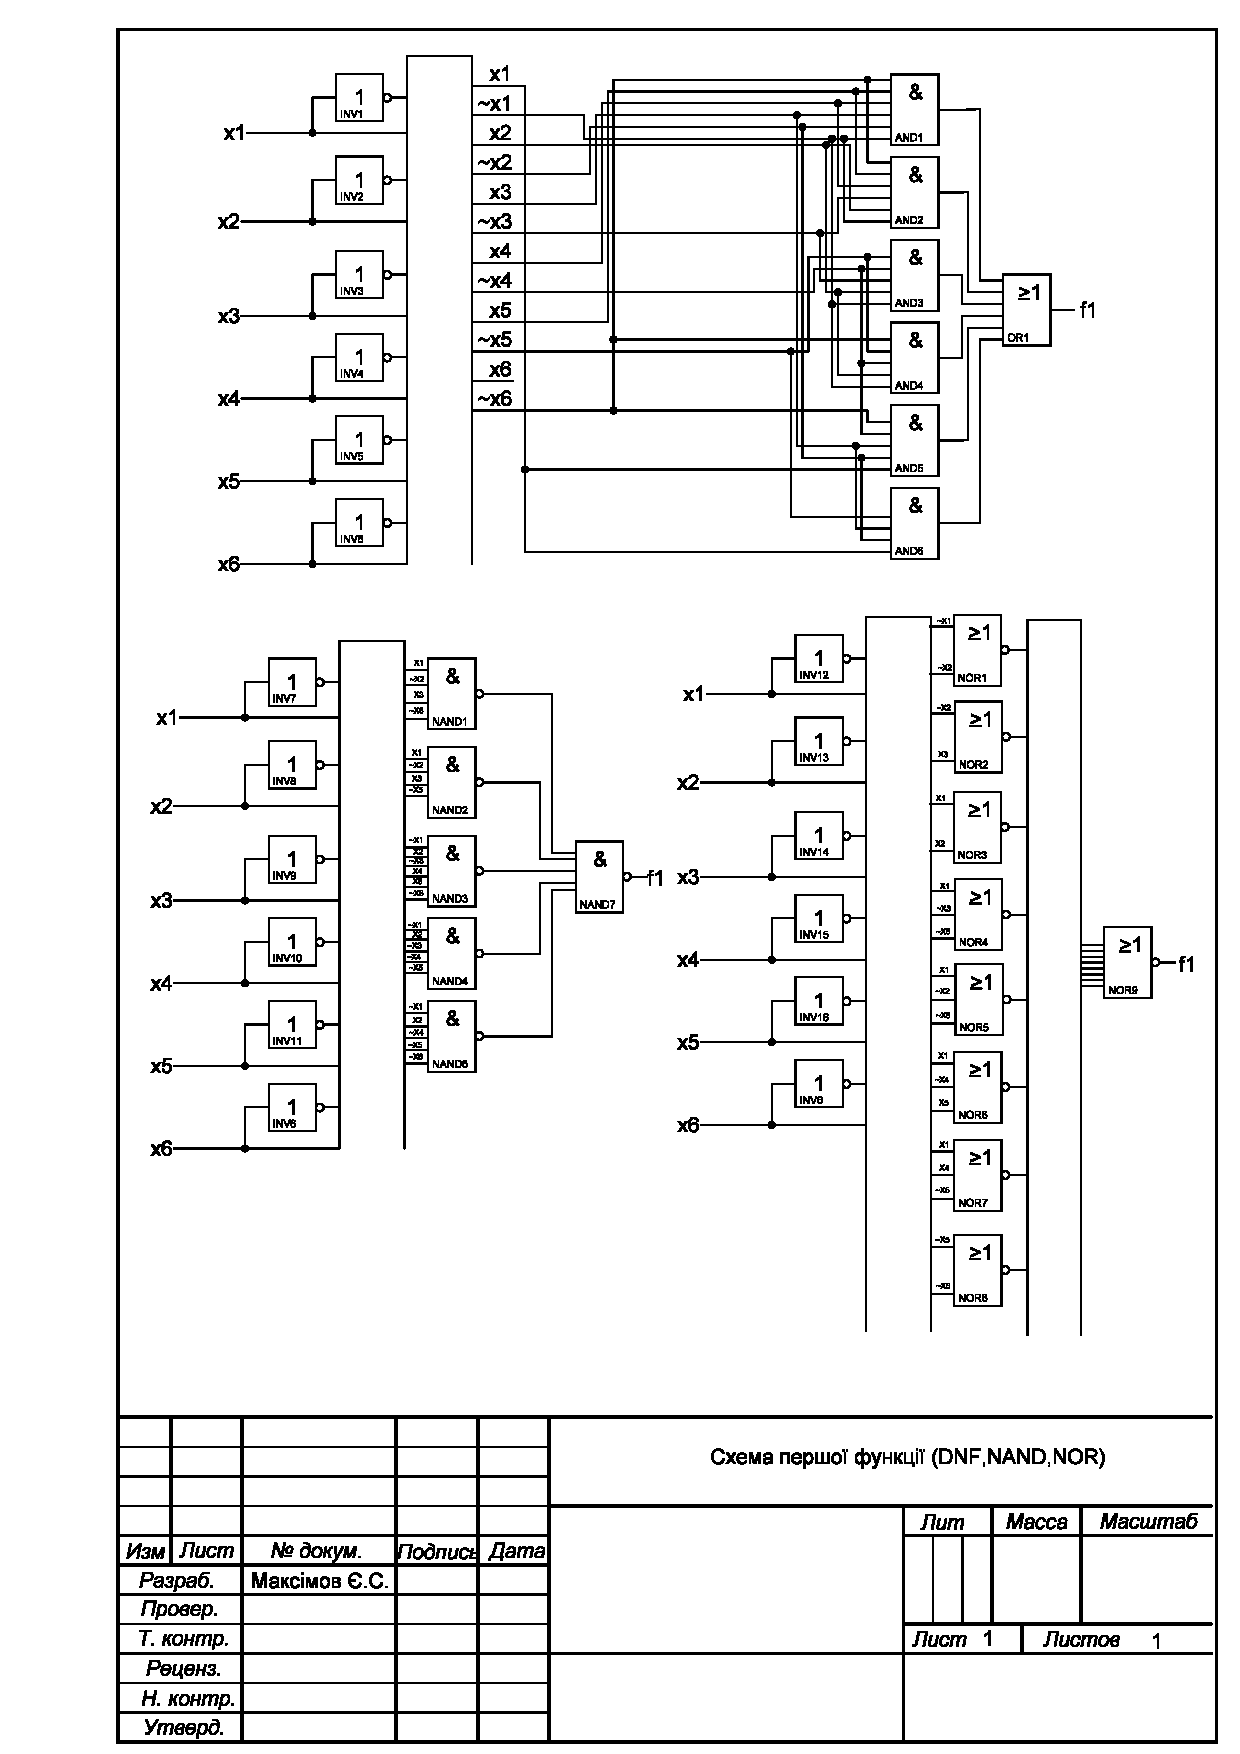
\includepdf[pages=-]{scheme_11.pdf}
\newpage
\section{Друга функція}
\begin{center}
\tablefirsthead{
\hline 
$N$&$X_{1}$ & $X_{2}$ & $X_{3}$ & $X_{4}$ & $X_{5}$ & $X_{6}$ & $F_{2}$ \\ }
\tablehead{
\hline 
$N$&$X_{1}$ & $X_{2}$ & $X_{3}$ & $X_{4}$ & $X_{5}$ & $X_{6}$ & $F_{2}$ \\ }
\tabletail{\hline}
\tablecaption{Таблиця істинності другої логічної функції}
\label{tab:tt_2}
\begin{supertabular}{|c|c|c|c|c|c|c|c|}
\hline
0&0 & 0 & 0 & 0 & 0 & 0 & 1 \\ 
\hline
1&0 & 0 & 0 & 0 & 0 & 1 & 1 \\ 
\hline
2&0 & 0 & 0 & 0 & 1 & 0 & 1 \\ 
\hline
3&0 & 0 & 0 & 0 & 1 & 1 & 1 \\ 
\hline
4&0 & 0 & 0 & 1 & 0 & 0 & 1 \\ 
\hline
5&0 & 0 & 0 & 1 & 0 & 1 & 1 \\ 
\hline
6&0 & 0 & 0 & 1 & 1 & 0 & 1 \\ 
\hline
7&0 & 0 & 0 & 1 & 1 & 1 & 1 \\ 
\hline
8&0 & 0 & 1 & 0 & 0 & 0 & 1 \\ 
\hline
9&0 & 0 & 1 & 0 & 0 & 1 & 1 \\ 
\hline
10&0 & 0 & 1 & 0 & 1 & 0 & 1 \\ 
\hline
11&0 & 0 & 1 & 0 & 1 & 1 & 1 \\ 
\hline
12&0 & 0 & 1 & 1 & 0 & 0 & 1 \\ 
\hline
13&0 & 0 & 1 & 1 & 0 & 1 & 0 \\ 
\hline
14&0 & 0 & 1 & 1 & 1 & 0 & 1 \\ 
\hline
15&0 & 0 & 1 & 1 & 1 & 1 & 0 \\ 
\hline
16&0 & 1 & 0 & 0 & 0 & 0 & 1 \\ 
\hline
17&0 & 1 & 0 & 0 & 0 & 1 & 0 \\ 
\hline
18&0 & 1 & 0 & 0 & 1 & 0 & 1 \\ 
\hline
19&0 & 1 & 0 & 0 & 1 & 1 & 1 \\ 
\hline
20&0 & 1 & 0 & 1 & 0 & 0 & 0 \\ 
\hline
21&0 & 1 & 0 & 1 & 0 & 1 & 1 \\ 
\hline
22&0 & 1 & 0 & 1 & 1 & 0 & 0 \\ 
\hline
23&0 & 1 & 0 & 1 & 1 & 1 & 0 \\ 
\hline
24&0 & 1 & 1 & 0 & 0 & 0 & 0 \\ 
\hline
25&0 & 1 & 1 & 0 & 0 & 1 & 0 \\ 
\hline
26&0 & 1 & 1 & 0 & 1 & 0 & 1 \\ 
\hline
27&0 & 1 & 1 & 0 & 1 & 1 & 1 \\ 
\hline
28&0 & 1 & 1 & 1 & 0 & 0 & 1 \\ 
\hline
29&0 & 1 & 1 & 1 & 0 & 1 & 1 \\ 
\hline
30&0 & 1 & 1 & 1 & 1 & 0 & 1 \\ 
\hline
31&0 & 1 & 1 & 1 & 1 & 1 & 1 \\ 
\hline
32&1 & 0 & 0 & 0 & 0 & 0 & 1 \\ 
\hline
33&1 & 0 & 0 & 0 & 0 & 1 & 1 \\ 
\hline
34&1 & 0 & 0 & 0 & 1 & 0 & 1 \\ 
\hline
35&1 & 0 & 0 & 0 & 1 & 1 & 1 \\ 
\hline
36&1 & 0 & 0 & 1 & 0 & 0 & 1 \\ 
\hline
37&1 & 0 & 0 & 1 & 0 & 1 & 1 \\ 
\hline
38&1 & 0 & 0 & 1 & 1 & 0 & 1 \\ 
\hline
39&1 & 0 & 0 & 1 & 1 & 1 & 1 \\ 
\hline
40&1 & 0 & 1 & 0 & 0 & 0 & 1 \\ 
\hline
41&1 & 0 & 1 & 0 & 0 & 1 & 1 \\ 
\hline
42&1 & 0 & 1 & 0 & 1 & 0 & 1 \\ 
\hline
43&1 & 0 & 1 & 0 & 1 & 1 & 0 \\ 
\hline
44&1 & 0 & 1 & 1 & 0 & 0 & 0 \\ 
\hline
45&1 & 0 & 1 & 1 & 0 & 1 & 1 \\ 
\hline
46&1 & 0 & 1 & 1 & 1 & 0 & 0 \\ 
\hline
47&1 & 0 & 1 & 1 & 1 & 1 & 0 \\ 
\hline
48&1 & 1 & 0 & 0 & 0 & 0 & 1 \\ 
\hline
49&1 & 1 & 0 & 0 & 0 & 1 & 1 \\ 
\hline
50&1 & 1 & 0 & 0 & 1 & 0 & 1 \\ 
\hline
51&1 & 1 & 0 & 0 & 1 & 1 & 1 \\ 
\hline
52&1 & 1 & 0 & 1 & 0 & 0 & 1 \\ 
\hline
53&1 & 1 & 0 & 1 & 0 & 1 & 1 \\ 
\hline
54&1 & 1 & 0 & 1 & 1 & 0 & 1 \\ 
\hline
55&1 & 1 & 0 & 1 & 1 & 1 & 1 \\ 
\hline
56&1 & 1 & 1 & 0 & 0 & 0 & 1 \\ 
\hline
57&1 & 1 & 1 & 0 & 0 & 1 & 1 \\ 
\hline
58&1 & 1 & 1 & 0 & 1 & 0 & 1 \\ 
\hline
59&1 & 1 & 1 & 0 & 1 & 1 & 1 \\ 
\hline
60&1 & 1 & 1 & 1 & 0 & 0 & 1 \\ 
\hline
61&1 & 1 & 1 & 1 & 0 & 1 & 1 \\ 
\hline
62&1 & 1 & 1 & 1 & 1 & 0 & 1 \\ 
\hline
63&1 & 1 & 1 & 1 & 1 & 1 & 1 \\ 
\hline
\end{supertabular}
\end{center}
\newpage
\subsection{Мінімізована логічна функція та базиси І-НЕ(NAND) та АБО-НЕ(NOR)}
\begin{itemize}
\item Мінімізована логічна функція(КНФ):

$F_{2 CNF}=(\neg X_{1}\lor X_{2}\lor \neg X_{3}\lor \neg X_{4}\lor X_{6})\land (\neg X_{1}\lor X_{2}\lor \neg X_{3}\lor \neg X_{5}\lor \neg X_{6})\land (X_{1}\lor \neg X_{2}\lor \neg X_{3}\lor X_{4}\lor X_{5})\land (X_{1}\lor \neg X_{2}\lor X_{3}\lor \neg X_{4}\lor \neg X_{5})\land (X_{1}\lor \neg X_{2}\lor X_{3}\lor \neg X_{4}\lor X_{6})\land (X_{1}\lor \neg X_{2}\lor X_{4}\lor X_{5}\lor \neg X_{6})\land (X_{1}\lor X_{2}\lor \neg X_{3}\lor \neg X_{4}\lor \neg X_{6})$;
\item Базис І-НЕ(NAND):

$F_{2 NAND}=(X_{1}\uparrow X_{2})\uparrow (X_{1}\uparrow \neg X_{4}\uparrow \neg X_{6})\uparrow (X_{1}\uparrow \neg X_{5}\uparrow X_{6})\uparrow (\neg X_{1}\uparrow \neg X_{2}\uparrow \neg X_{4})\uparrow (\neg X_{1}\uparrow X_{3}\uparrow X_{4}\uparrow \neg X_{6})\uparrow (\neg X_{1}\uparrow \neg X_{4}\uparrow X_{5})\uparrow (X_{2}\uparrow X_{3}\uparrow X_{4})\uparrow (X_{2}\uparrow X_{4}\uparrow \neg X_{5}\uparrow X_{6})\uparrow (\neg X_{2}\uparrow \neg X_{3})\uparrow (\neg X_{3}\uparrow \neg X_{4}\uparrow \neg X_{6})$;
\item Базис АБО-НЕ(NOR):

$F_{2 NOR}=(\neg X_{1}\downarrow X_{2}\downarrow\neg X_{3}\downarrow\neg X_{4}\downarrow X_{6})\downarrow(\neg X_{1}\downarrow X_{2}\downarrow\neg X_{3}\downarrow\neg X_{5}\downarrow\neg X_{6})\downarrow(X_{1}\downarrow\neg X_{2}\downarrow\neg X_{3}\downarrow X_{4}\downarrow X_{5})\downarrow(X_{1}\downarrow\neg X_{2}\downarrow X_{3}\downarrow\neg X_{4}\downarrow\neg X_{5})\downarrow(X_{1}\downarrow\neg X_{2}\downarrow X_{3}\downarrow\neg X_{4}\downarrow X_{6})\downarrow(X_{1}\downarrow\neg X_{2}\downarrow X_{4}\downarrow X_{5}\downarrow\neg X_{6})\downarrow(X_{1}\downarrow X_{2}\downarrow\neg X_{3}\downarrow\neg X_{4}\downarrow\neg X_{6})$.
\end{itemize}
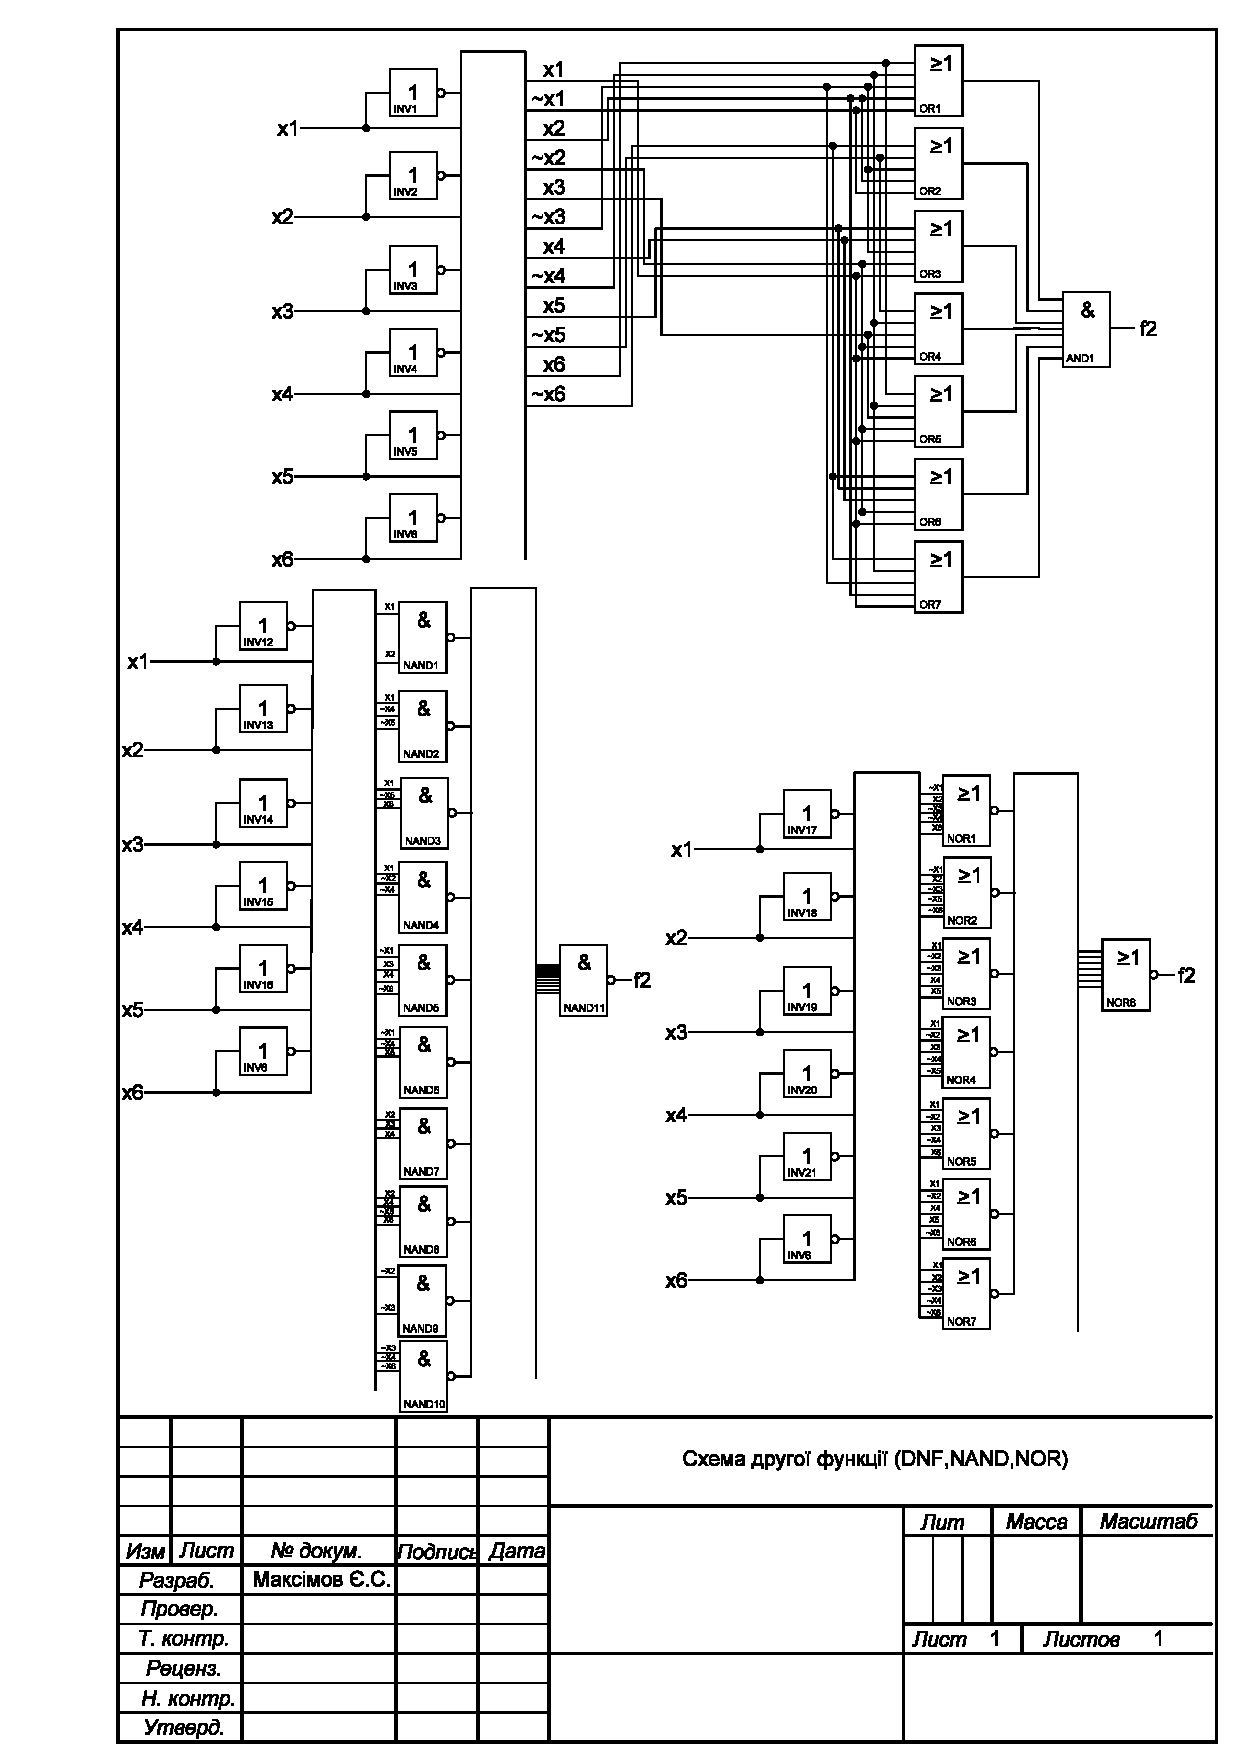
\includepdf[pages=-]{scheme_12.pdf}
\newpage
\chapter{Друге завдання}
\section{Характеристики дешифратора згідно варіанту}
\begin{center}
\begin{table}[h!]
\begin{tabu}{ | X[-3,l] | X[6,l] | X[6,l] | X[-3,l]|}
\hline
$N=19$ & $K_{1}=4$ & $K_{2}=3$  & $K_{3}=5$ \\
\hline
$L=4$,\newline згідно(\ref{eq:decoder_L}) & $l_{1}=1$, \newline згідно(\ref{eq:decoder_N}) & $l_{2}=0$,\newline згідно(\ref{eq:decoder_N}) & $l_{3}=3$,\newline згідно(\ref{eq:decoder_N}) \\
\hline
$A_{1}=182$ & $1129_{10}$ & $1311_{10}$ &  \\
\hline
& $10001101001_{2}$ & $10100011111_{2}$ &  \\
\hline
$A_{2}=173$ & $443147_{10}$ & $443320_{10}$ &   \\
\hline
& $1101100001100001011_{2}$ & $1101100001110111000_{2}$ &  \\
\hline
\end{tabu}
\vspace{6mm}\\
\caption{Характеристики дешифратора згідно варіанту}\label{tab:decoder_spec}
\end{table}
\end{center}
\subsection{Таблиця адресних просторів та схема багатоступеневого неповного дешифратора}
\begin{center}
\begin{table}[h!]
\begin{tabu}{ | X[-3,l] | X[-3,l] | X[-3,l] | X[-3,l] |X[-3,l] |}
\hline
N & 18,17,16,15 & 14,13,12,11,10 & 9,8,7,6,5 & 4,3,2,1,0 \\
 \hline
$A_{1e}$ & 0000 & 00001 & 01000 & 11111  \\
\hline
$A_{1a}$ &  0 & 1  &  8-3 & 31-9  \\
\hline
$A_{1b}$ & 0000 & 00001 & 00011 & 01001   \\
\hline
$A_{2e}$ & 1101 & 10000 & 11101 & 11000  \\
\hline
$A_{2a}$ & 13 & 16 & 29-24 & 24-11  \\
\hline
$A_{2b}$ & 1101 & 10000 & 11000 & 01011  \\
\hline
\end{tabu}
\vspace{6mm}\\
\caption{Таблиця адресних просторів}\label{tab:decoder_addr}
\end{table}
\end{center}
%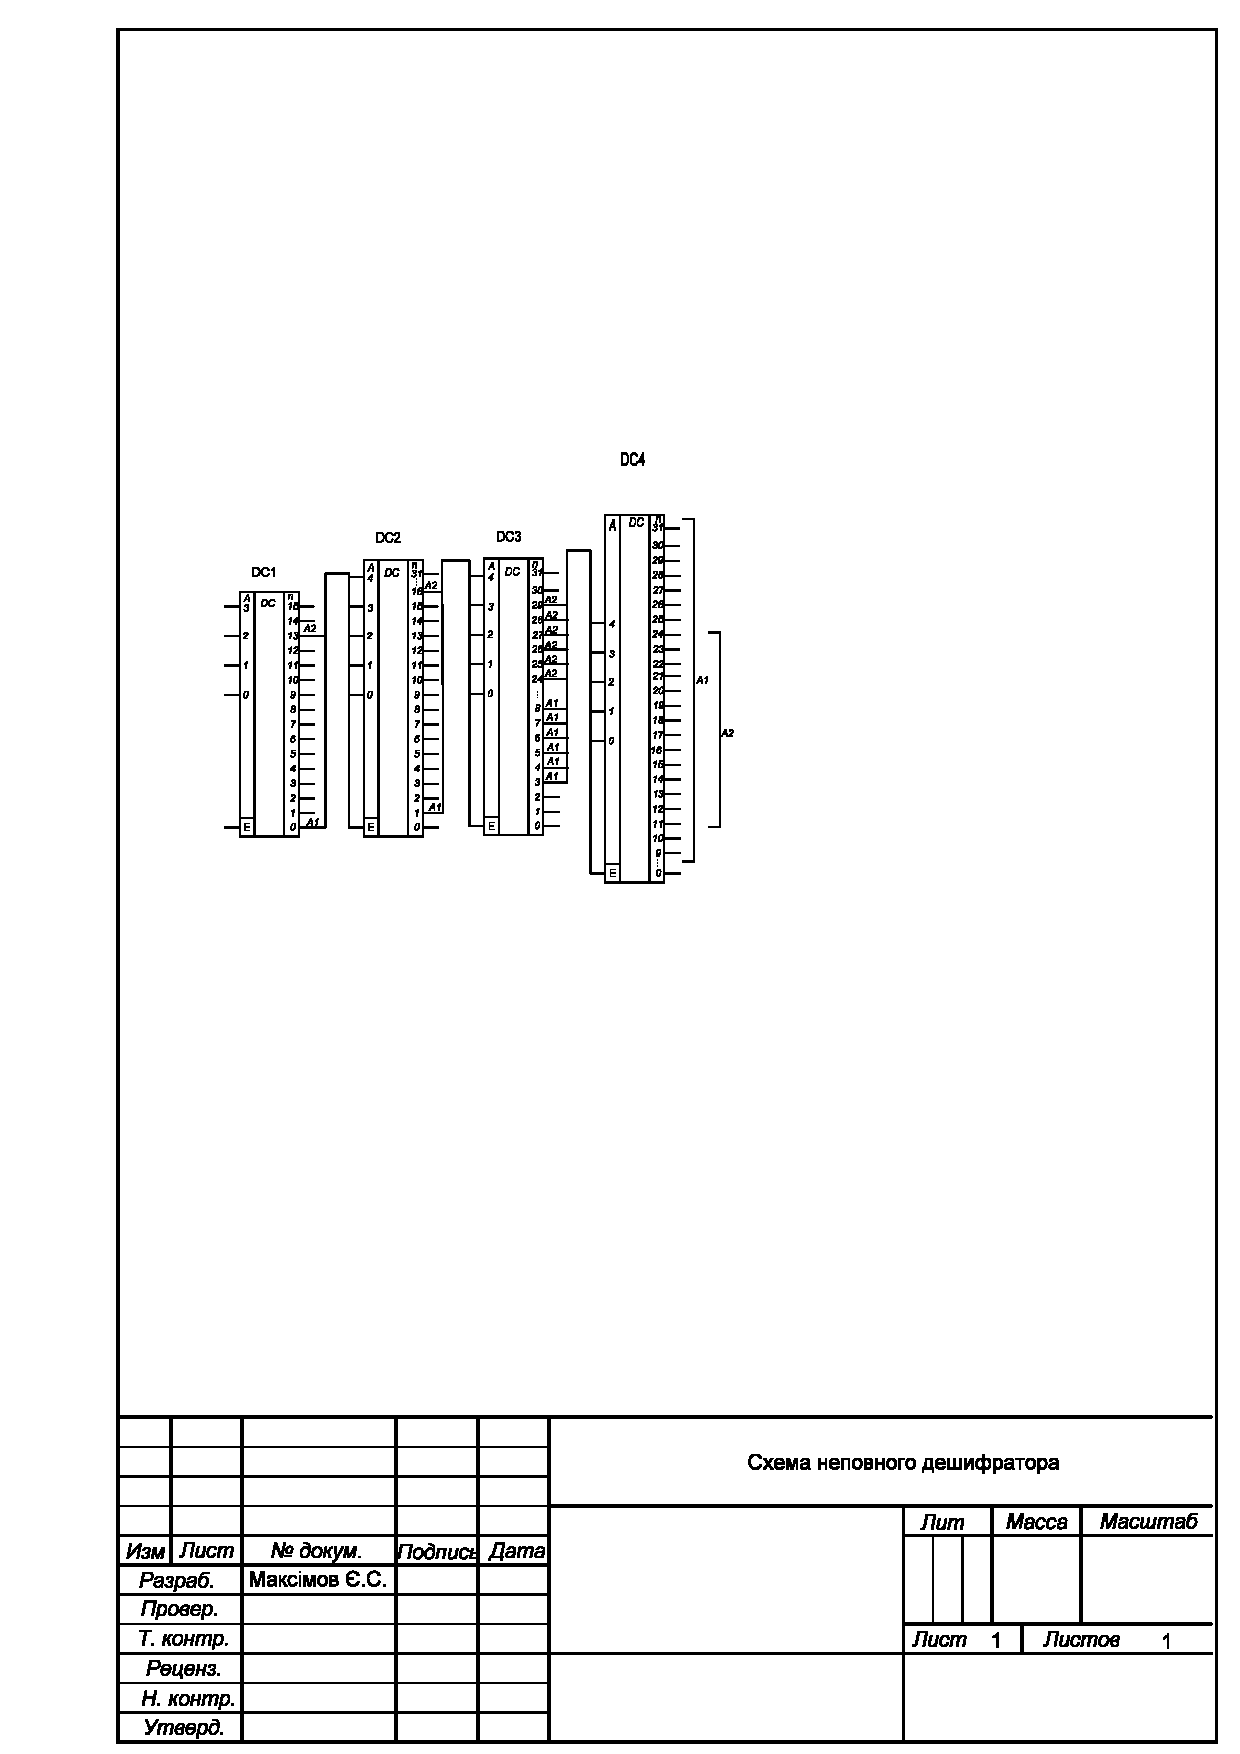
\includepdf[pages=-]{scheme_2.pdf}
\newpage
\section{Апаратні витрати на побудову дешифратора}
За данними таблиці \ref{tab:decoder_spec} та формулами (\ref{eq:decoder_n1}),(\ref{eq:decoder_nj}) маємо таку кількість дешифраторів $\sum n=1+2^{4}+2^{4}*2^{5}+2^{4}*2^{5}*2^{5}+2^{4}*2^{5}*2^{5}*2^{5}=1+2^{4}+2^{9}+2^{14}+2^{19}>2^{N}$
\newpage
\chapter{Висновок}
Ми використовуємо багато складних електричних пристроїв, наприклад ЕОМ, тому розробка цифрових пристроїв важлива частина інформаційного століття. Під час виконання роботи я познайомився з процесом оптимізації логічних пристроїв, проектування каскадних цифрових пристроїв та отримав важні засади розуміння функціонування цифрових пристроїв а, також використав на практиці знання здобуті при вивченні дисципліни «Технології проектування ком'ютерних систем».